\documentclass[size=A4]{scrreprt}

\usepackage[utf8x]{inputenc}
\usepackage[ngerman]{babel}
\usepackage{listings}
\usepackage{graphicx}
\usepackage{color}
\usepackage{todonotes}
\usepackage{mathtools}

\definecolor{mygreen}{rgb}{0.08,0.35,0}
\definecolor{mygray}{rgb}{0.9,0.9,0.9}
\definecolor{mymauve}{rgb}{0.58,0,0.82}

\title{Ein Vergleich der Verifikationswerkzeuge Verifast und Frama-C}
\author{Georg Wächter\\Humboldt Universität zu Berlin}
\date{Dezember 2013}

\lstset{
  backgroundcolor=\color{mygray}, 
  basicstyle=\ttfamily\small,     
  breakatwhitespace=false,      
  breaklines=true,                
  captionpos=b,                  
  commentstyle=\color{mygreen},    
  extendedchars=true,       
  frame=none,                 
  keywordstyle=\color{blue},     
  language=Octave,               
  morekeywords={bool},       
  numbers=left,               
  numbersep=5pt,                
  numberstyle=\color{black},
  rulecolor=\color{black},  
  stepnumber=1,       
  stringstyle=\color{mymauve},  
  tabsize=2,   
  columns=fixed,                  
}

\begin{document}

\maketitle
\tableofcontents

\chapter{Einleitung}

\section{Aufgabenstellung und Durchführung}
\label{sec:aufgabenstellung}
Diese Arbeit vergleicht die statischen Verifikationswerkzeuge Verifast\footnote{
\url{http://people.cs.kuleuven.be/~bart.jacobs/verifast/}} und ACSL\footnote{\url{http://frama-c.com/acsl.html}} 
in Kombination mit Frama-C\footnote{\url{http://frama-c.com}}. 
Der Fokus liegt dabei auf einfachen Algorithmen, die mit Arrays arbeiten ohne sie zu verändern.
Dabei wird die Lesbarkeit, Ausdrucksstärke sowie der notwendige manuelle Aufwand der Verifikation betrachtet.
Für den praktischen Einsatz wichtige Faktoren werden ebenso untersucht. Das sind insbesondere die verfügbare 
Dokumentation, die Integration in den Entwicklungsprozess und die Geschwindigkeit der Werkzeuge.
\newline
\newline
Als durchgängiges Beispiel dient in dieser Arbeit der standardisierte mismatch-Algorithmus\footnote{siehe
\url{http://msdn.microsoft.com/de-de/library/f0bsxbk9.aspx}} aus
der C++ Standard-Bibliothek. Die Grundlage für spätere Formalisierung ist die folgende vereinfachte\footnote{es
wird auf Iteratoren und eine selbst definierte Vergleichsfunktion verzichtet} Signatur und 
die dazugehörige informelle Spezifikation:

\lstset{frame=none, numbers=none}    
\lstinputlisting[language=C]{codes/mismatch_signature.c}
\lstset{frame=single, numbers=left}

\noindent \emph{Vergleicht die Elemente der beiden Arrays beginnend bei 0 bis einschließlich size - 1 und gibt den
Index der ersten Elemente zurück, die sich unterscheiden. Sind alle Elemente gleich, gibt der Algorithmus
size - die Länge der Liste - zurück.}
\newline
\newline
Auf Grund des einfachen Beispiels hat der Vergleich nur eine begrenzte Aussagekraft, denn es werden nicht alle
Spracheigenschaften von Verifast bzw. ACSL gezeigt und verglichen. Zudem kommt hinzu, dass sich beide Werkzeuge
kontinuierlich - in ihre jeweils eigene Richtung - weiterentwickeln. Es wird darum immer Anwendungsfälle geben,
in denen ein Werkzeug dem anderen überlegen ist oder sogar alternativlos ist.


\section{Verifast}
\label{sec:verifast}



KU Löwen university, by bart jacobs


for C and java


functional correctness


seperation logic - angepasste hoare logic


malloc/free - keien speicherlöscher


multithreading .. z.B. lock free datenstrukturen

kein eigener name für die sprache, darum wird immer nur von verifast gesprochen


industrieeinsatz

\section{Frama-C}
\label{acsl-und-frama-c}

ansi/iso-c specification language


zusammen mit verifast teil des STANCE projekts

\section{Zielgruppe}
\label{sec:zielgruppe}

Für das Verstehen der Arbeit sollte der Leser die Grundlagen der Programmiersprache C beherrschen.
sowie theoretische Kenntnisse zur Aussagen- und Prädikatenlogik besitzen.
Konkrete Erfahrungen mit ACSL und Frama-C sind hilfreich, da beim Vergleich der Werkzeuge an vielen
Stellen Verifast detaillierter als ACSL erläutert wird. Die Arbeit ist darum auch als Einstieg in Verifast
für ACSL-Nutzer geeignet und ausgelegt.

 



\chapter{Theoretische Grundlagen}

In diesem Kapitel werden die theoretischen Grundlagen der beiden Verifikationswerkzeuge kurz erläutert. Dabei wird bewusst
auf ausführliche Formalismen verzichtet, diese können in den Quellen bei Bedarf nachgelesen werden.

Als erstes wird der Hoare-Kalkül beschrieben - die Grundlage der Softwareverifikation von Frama-C als auch VeriFast.
Anschließend werden die Begriffe der partiellen und totalen Korrekheit im Zusammenhang mit der Terminierung eines Programms
eingeführt. Der letzte Abschnitt widmet sich der Separierungslogik - der theoretischen Basis für die Verifizierung
mit VeriFast.

\section{Hoare-Kalkül}

Der Hoare-Kalkül ist ein formales System zum Beweisen der Korrektheit von Programmen. Es verwendet eine Reihe logischer
Regeln und Axiome, die direkt auf den Quellcode angewendet werden und mit sogenannten Hoare-Tripeln arbeiten. Ein solches
Tripel beschreibt den Zustand vor und nach der Ausführung eines Programmteils mit Hilfe von prädikatenlogischen
Formeln.
\begin{displaymath}
\{P\} \: S \: \{Q\}
\end{displaymath}
Die Formel P gilt vor, Q hingegen nach der Ausführung von S. Damit kann nun die Ableitungsregel zur Komposition von
zwei aufeinander folgenden Programmabschnitten aufgestellt werden:
\begin{displaymath}
\frac{\{P\} \:S\: \{R\} \:, \: \{R\} \: T \: \{Q\}}{\{P\}\: S; T \: \{Q\}}
\end{displaymath}
Die Regeln besagen, dass die unter dem Strich stehende Aussage aus der über dem Strich notierten Aussage folgt. In diesem
Fall beschreibt die Regel die Verkettung zweier Tripel.

Da die im Fokus stehenden Algorithmen mit Schleifen arbeiten, sei hier noch die Iterationsregel gezeigt, die auf While-Schleifen
bzw. auf For-Schleifen im C-Code angewendet wird: 
\begin{displaymath}
\frac{\{I \land B\} \:S\: \{I\}}{\{I\}\: while(B)\: S\: \{I \land \neg B\}}
\end{displaymath}
I bezeichnet die Schleifeninvariante, S den Schleifenkörper und B die Eintrittsbedingung. Kann nachgewiesen werden,
dass S die Invariante erhält und vor der Ausführung B und~I wahr sind, dann gilt die unter dem Strich stehende Aussage: Nachdem
die Schleife durchlaufen ist, gilt nicht B und weiterhin die Invariante. B und S sind direkt aus dem Quellcode entnommen, 
die Schleifeninvariante hingegen muss bei der Verifizierung  manuell angegeben werden (siehe dazu den Abschnitt über 
Schleifeninvarianten im Kapitel 4).

Für die Verifizierung müssen nun alle Regeln auf den Quellcode angewendet werden. Eine von Frama-C verwendete Variation des Hoare-Kalküls
stellt das System der schwächsten Vorbedingungen (engl. weakest preconditions) dar. Dabei findet eine Rückwärtsanalyse
des Quellcodes statt. Begonnen wird mit den zu beweisenden Nachbedingungen. In jedem Schritt wird dann die schwächste Vorbedingung
abgeleitet, sodass am Ende zu beweisen ist, dass die zuletzt berechnete Vorbedingung aus der Vorbedingung des Kontrakts folgt.
Ist dieses Vorgehen erfolgreich, so erfüllt der Quellcode die gegebene Spezifikation aus Vor- und Nachbedingung.

\section{Terminierung}

Mit Hilfe des Hoare-Kalküls lässt sich nicht nachweisen, dass ein Programm terminiert, d.h. nach endlich vielen Schritten 
beendet ist. Man spricht deshalb von der partiellen Korrektheit, da das Programm nur dann das gewünschte 
Verhalten zeigt, wenn es auch tatsächlich zum Ende kommt.

Die Iterationsregel lässt sich z.B. auch dann anwenden, wenn es sich um eine Endlosschleife handelt. Der Nachweis,
dass die Schleife tatsächlich terminiert, ist zusätzlich zu erbringen. 

Die folgende erweiterte Iterationsregel erbringt bei Anwendung genau diesen Beweis. Für die entsprechende Schleife ist damit, die
sogenannte totale Korrektheit gezeigt:
\begin{displaymath}
\frac{\{I \land B \land t = z \} \:S\: \{I \land t < z\}, I \implies t \geq 0}{\{I\}\: while(B)\: S\: \{I \land \neg B\}}
\end{displaymath}

Diese erweiterte Regel ergänzt die als \lstinline{t} bezeichnete Schleifenvariante. Durch die zusätzliche Bedingung, dass aus der gültigen Invariante
eine positive Variante folgt, ergibt sich die Terminierung der Schleife. Denn in jedem Schleifendurchlauf verringert sich die Variante,
sodass letztendlich irgendwann ein Ende erreicht sein muss\footnote{Die Variante t könnte in diesem Fall mit natürlichen Zahlen arbeiten,
das Prinzip ist aber nicht darauf beschränkt, siehe dazu die formalen Ausführungen in \cite{floyd}[Seite 31].}.

Der Nachweis der totalen Korrektheit wird in dieser Arbeit für die vorgestellten einfachen Algorithmen angestrebt.
Allerdings ist es nicht möglich die Terminierung für beliebige Algorithmen zu beweisen, da es sich um ein nicht entscheidbares 
Problem handelt\footnote{Der Mathematiker Alan Turing hat bereits 1936 bewiesen, dass es keinen Algorithmus gibt, der 
entscheiden kann, dass ein beliebiger Algorithmus zum Ende kommt\cite{turing}[Seite 230-265].}.

\section{Separierungslogik}
\label{sec:theorie:seperation-logic}

Die Separierungslogik ist eine Erweiterung des Hoare-Kalküls, die weitergehende Aussagen über den Speicherinhalt
und den Zugriff darauf erlaubt. Die Bedeutung des Hoare-Tripels wird dazu etwas erweitert -- der Programmcode des
betrachteten Tripels darf nur noch auf den Speicher zugreifen, der in der Vorbedingung erwähnt oder aber im Code
allokiert wurde\cite{reynolds-2002}[Kapitel 4].

Außerdem wird die von Hoare definierte zugrunde liegende Programmiersprache erweitert, um Befehle zum Anfordern (engl. allocate), 
Löschen, Manipulieren und Auslesen des Speichers. Der Ausführungszustand wird um zwei neue Komponenten erweitert, damit 
diese Aktionen abgebildet werden können: Der dynamische Speicherbereich (engl. heap) verknüpft Adressen mit ihren
Werten; die lokalen Variablen (engl. store/stack) assoziieren die Namen der Variablen mit ihren Inhalten. 

Die neu eingeführten Konstrukte sind bewusst stark angelehnt an die maschinennahen Konzepte der Zeigerarithmetik sowie des
Stapelspeichers. Somit ist die Anwendung der Logik auf C-Programme leicht möglich.

Damit Vor- und Nachbedingungen Aussagen über den Speicher treffen können, erweitert die Separierungslogik die
von Hoare verwendete Prädikatenlogik um folgende Operatoren bzw. Atome: 
\begin{align*}
\langle Aussage \rangle & ::= \dots \\
& \begin{array}{l r}
  | \: \textbf{emp} & \textrm{leerer Speicher}\\
  | \: \langle Ausdruck \rangle \to \langle Ausdruck \rangle & \textrm{einzelner Wert im Speicher}\\
  | \: \langle Aussage \rangle \ast \langle Aussage \rangle & \textrm{disjunkte Speicherbereiche, Konjunktion}\\
  | \: \langle Aussage \rangle -\!\! \ast \langle Aussage \rangle & \textrm{disjunkte Speicherbereiche, Implikation}\\
\end{array}
\end{align*}
Insbesondere die spezielle Konjunktion ist an dieser Stelle wichtig, da sie auch in \mbox{VeriFast} eine wichtige Rolle spielt.
Sie stellt sicher, dass beide Aussagen zutreffen und die entsprechenden Speicherbereiche disjunkt sind. 

Das folgende Hoare-Tripel zeigt ein Beispiel für die Anwendung der Operatoren. Der gezeigte Programmabschnitt ist in C-Syntax
formuliert und demonstriert die Semantik des Konjunktions-Operators.
\begin{align*}
& \{a \to 5 \ast b \to 5 \} \\
& \text{*a = *a + *b;} \\
& \{a \to 10 \ast b \to 5\}
\end{align*}
Dieses Tripel wäre ungültig, wenn man eine einfache logische Konjunktion wie aus der Aussagenlogik einsetzen würde. Dann
wäre nicht auszuschließen, dass die Variablen \lstinline{a} und \lstinline{b} dieselbe Speicheradresse meinen.

VeriFast unterstützt außerdem das Konzept der geteilten Speicherzugriffe (engl. fractional permissions). Das
ist eine Ergänzung zur Separierungslogik mit der das Aufsplitten von Lesezugriffen für Speicherbereiche möglich ist\cite{concurrent}.
Damit ist auch das Formalisieren und Beweisen paralleler Programme möglich.  

Der Funktionsumfang der Annotationssprache für VeriFast ist also nicht deckungsgleich mit dem aus der Arbeit von Reynolds.
Teilweise wurde die Sprache reduziert und an anderen Stellen erweitert, die Nutzung von Quantoren ist in VeriFast beispielsweise
nicht erlaubt.


\chapter{Vergleich grundlegender Konzepte}

\section{Spezifikationen und Prädikate für equal}
\label{sec:design-by-contract}
\subsection{Design by Contract}

Bei der formalen Verifikation geht es darum sicherzustellen, dass ein entsprechendes Stück Software
funktional korrekt ist. Das wird erreicht, in dem man die Bausteine der Sprache - in C sind es zum Beispiel die Methoden 
oder Strukturen -
Stück für Stück formalisiert und verifiziert. Die Signatur einer Methode stellt bereits einen einfachen Vertrag zwischen
Aufrufenden und Aufrufer dar - Parameteranzahl und ihre Typen sind festgelegt, genauso wie der Rückgabewert.
Um auch die funktionalen Aspekte der Methode zu beschreiben, wird diese Vereinbarung um sogenannte Vor- und Nachbedingungen erweitert.
Diese beschreiben das Resultat der Methode sowie notwendige Annahmen, die vor dem Aufrufen der Methode gegeben sein müssen. 

Somit entstehen exakte vollständig formalisierte Bausteine, die keinen Raum für Ungenauigkeiten oder Interpretationen zulassen.
Diese Herangehensweise nennt sich Design by Contract und ist die Grundidee der meisten Verifikationswerkzeuge.



\subsection{ACSL-Spezifikation für equal}
\label{sec:design-by-contract:acsl-spezifikation}

Nachfolgend ist ein einfaches Beispiel einer ACSL-Funktions-Spezifikation dargestellt.
Die Funktion equal prüft zwei Ganzzahlen-Arrays auf Gleichheit:

\lstinputlisting[language=C]{codes/equal_contract_acsl.c}

Der spezielle @-Präfix in Zeile 1 signalisiert dem Verifikationswerkzeug, 
dass der folgende Kommentarblock als Verifikations-Annotation zu interpretieren ist. Normale C-Compiler hingegen
ignorieren den Kommentar.

Die Vorbedingungen sind in Zeile 2 und 3 zu finden: \lstinline{IsValidRange} ist ein Prädikat, welches hier sicherstellt,
dass die Zeiger \lstinline{a} und \lstinline{b} gültig sind und auf den Speicherbereich \lstinline{a[0..n]} 
(von \lstinline{a[0]} bis \lstinline{a[n-1]}) bzw. \lstinline{b[0..n]} zugegriffen 
werden darf. Zusätzlich verbietet das Prädikat negative Array-Größen.

Die \lstinline{\assigns}-Klausel beschreibt potenzielle Seiteneffekte. Da es sich bei equal um eine nicht mutierende
Funktion handelt, wird hier kein Speicher verändert.

Der Rückgabewert, identifiziert durch \lstinline{\result}, wird durch die Nachbedingung in Zeile 7 definiert. Er ist genau dann
wahr, wenn die Ganzzahlen-Arrays \lstinline{a[0..n]} und \lstinline{b[0..n]} elementweise gleich sind. Ansonsten ist der 
zurückgegebene Bool-Wert falsch. 

Erreicht wird dies mit Hilfe des Prädikats \lstinline{IsEqual}. Dieses wiederum
nutzt folgende Aussage in Prädikatenlogik (erster Stufe mit Identifikation), um zu definieren wann genau 
zwei Arrays \lstinline{a} und \lstinline{b} der Länge \lstinline{n} gleich sind:
\[IsEqual(a, n, b) \equiv \forall(i) (0 \leq i < n \rightarrow a[i] = b[i])\]

Weitere Details zur allgemeinen Funktionsweise als auch speziell zu diesen Prädikaten siehe
\ref{sec:design-by-contract:predicates}.



\subsection{Variante mit Verifast}
\label{sec:design-by-contract:verifast-variante}

Als Vergleich nun eine semantisch identische Spezifikation in Verifast:

\lstinputlisting[language=C]{codes/equal_contract_verifast.c}

\todo{vergleich mit valid aus acsl einbringen, speziell mit valid array notation}
Als erstes fällt die unterschiedliche Platzierung der Annotation auf: In Verifast werden die 
Annotations-Kommentare nach der Signatur eingefügt. Außerdem müssen alle Vor- und Nachbedingungen
in nur einer \lstinline{requires} bzw. \lstinline{ensures}-Anweisung zusammengefasst werden.

Eine \lstinline{assigns}-Klausel gibt es zudem auch nicht. Dennoch ist zu erkennen, dass es sich um einen 
nicht-mutierenden Algorithmus handelt. Anders als in ACSL wird nicht explizit angegeben ob und auf welche 
Speicherstellen zugegriffen werden darf. Stattdessen wird eine Aussage über den Speicherinhalt selbst getroffen.

Um Aussagen über den Speicherinhalt mit logischen Aussagen zu verbinden, gibt es in Verifast die spezielle 
Konjunktion \lstinline{&*&}. In diesem Beispiel wird hier z.B. die Vorbedingung \lstinline{n >= 0} mit Aussagen
zu den Speicherbereichen \lstinline{a[0..n]} und \lstinline{b[0..n]} verknüpft.

Der \lstinline{x |-> y} Operator bedeutet dabei, dass die Speicherstelle \lstinline{x} den Inhalt \lstinline{y} hat.
Unbekannte Werte werden per Mustererkennung (engl. pattern matching) ergänzt. Die Klausel
\lstinline{a[0..n] |-> ?al} hat damit zwei Aufgaben: Der erste Teil stellt sicher, dass der Zeiger a und
der dahinterliegende Speicherbereich \lstinline{a[0..n]} gültig ist; der zweite identifiziert eben diesen 
Speicherbereich und bindet ihn an die Variable \lstinline{al}.
Verifast erlaubt es nun im Gegensatz zu ACSL auf diese Variablen auch in den Nachbedingungen zuzugreifen. Damit
hat man nun ein Mittel, mit dem man Seiteneffekte exakt beschreiben sowie Speicherbereiche vergleichen kann.

Die Klauseln \lstinline{a[0..n] |-> al} und \lstinline{b[0..n] |-> bl} in Zeile 3 stellen nun sicher, dass der
Speicher unverändert bleibt. Der Rückgabewert wird in Verifast mit \lstinline{result} (ohne vorangestellten 
Backslash wie in ACSL) bezeichnet. Der Ausdruck \lstinline{result == (al == bl)} bedeutet also, dass der von der Funktion
zurückgegebene Wert genau dann wahr ist, wenn die Inhalte der Speicherbereiche \lstinline{al} und \lstinline{bl} 
gleich sind.

Die Verifast-Spezifikation hat also tatsächlich die gleiche Semantik, erreicht dies aber wegen der zu Grunde
liegenden Seperation Logic auf eine andere Art und Weise.

\todo{erklären, dass speicher so grundlegend ist in verifast, dass der eingehende speicher immer explizit in der nachbedingung auftauchen muss - oder geleakt werden muss}

\todo{erklären, dass verwendung von acsl old nicht notwendig ist, da durch mustererkennung alte werte in variablen gecshrieben werden können, die auch in nachbedingung gültig sind}
 
\subsection{Einfache und rekursive Prädikate}
\label{sec:design-by-contract:predicates}

Prädikate sind ein grundlegendes Abstraktionsmittel zum Zusammenfassen und Wiederverwenden von logischen 
Formeln in ACSL und Verifast.

Weiter oben wurde das Prädikat \lstinline{IsEqual} definiert, hier sei nun exemplarisch die ACSL-Notation
für diese Aussage dargestellt:

\lstinputlisting[language=C]{codes/equal_predicate_acsl.c}

Die Annotation ist eine direkte Umsetzung der Formel von oben - die Interpretation ist klar verständlich für 
jeden, der prädikatenlogische Formeln lesen kann.

\todo{in acsl gibt es induktive prädikate, die ähnliches erlauben}
In Verifast sind neben solch einfachen Prädikaten auch rekursive möglich. Damit ergibt sich die Möglichkeit
sogar unbegrenzte Datenstrukturen zu beschreiben \todo{referenz auf verifast-tutorial seite 9, chapter 7}. In dieser
Arbeit sind allerdings nur Arrays mit bekannter Länge Untersuchungsgegenstand. Doch auch für diese sind
rekursive Prädikate in Verifast die natürliche Art der Beschreibung. Beispielsweise können Ganzzahl-Arrays
wie folgt definiert werden:

\lstinputlisting[language=C]{codes/int_array_verifast.c}
 
Das Prädikat verweist solange auf sich selbst bis \lstinline{count <= 0}. Dass jede Speicherstelle tatsächlich
gültig ist, stellt das in Verifast eingebaute Prädikat \lstinline{integer} sicher. In dieser Form ist das Prädikat
\lstinline{int_array} nun praktisch identisch mit der \lstinline{IsValidRange}-Variante aus der ACSL-Spezifikation, 
die in \ref{sec:design-by-contract:acsl-spezifikation} zu sehen war.

Auffällig ist an der Stelle noch die Verwendung des \lstinline{_}-Zeichens in Zeile 3. Wie in vielen anderen 
Sprachen auch bezeichnet es eine anonyme Variable, die an dieser Stelle zwar angegeben werden muss, aber deren 
Inhalt nicht weiter interessiert. 

Wird das \lstinline{integer} Prädikat ohne anonyme Variable verwendet, bedeutet der Aufruf von 
\lstinline{integer(start, ?s)} so viel wie \lstinline{*start |-> ?s}. Allerdings erlaubt Verifast
den Einsatz des \lstinline{|->} Operators nicht zusammen mit der Derefenzierung eines einzelnen
Ganzzahl-Wertes.

Tatsächlich ist der Einsatz des \lstinline{int_array(a, n)} Prädikats äquivalent mit der Schreibweise 
von \lstinline{a[0..n] |-> _}, denn Verifast behandelt die Array-Notation intern wie ein rekursives
Prädikat.

Eine erweiterte Fassung dieses Prädikats wird weiter unten in \todo{referenz detaillierter auflösen}
\ref{sec:abstrakte-datentypen} beschrieben.



\subsection{Reduzierte Spezifikationen: Robustheit als Ziel}
\label{sec:design-by-contract:partielle-korrektheit}

Das Ziel der in \ref{sec:design-by-contract:acsl-spezifikation} vorgestellten Spezifikation war die
vollständige funktionale Definition, damit kein Raum für Interpretationen frei bleibt. Allerdings ist
das nicht immer gewünscht: Soll die Robustheit der Software sichergestellt werden, so ist das Aufspüren 
von potenziellen Null-Zeiger-Ausnahmen oder Speicherlöchern das Ziel und nicht die funktionale
Korrektheit. Für ersteres reicht eine reduzierte Spezifikation - funktionale Aspekte werden dabei 
weggelassen oder ggf. vereinfacht:

\lstinputlisting[language=C]{codes/equal_partial_contract_verifast.c}
 
Diese Spezifikation ist immer noch korrekt für eine equal-Implementierung, stellt aber selber nur sicher,
dass die Zeiger gültig sind und auf den Speicherbereich zugegriffen werden darf. Der Rückgabewert sowie 
der nicht mutierender Charakter des Algorithmus ist nun nicht mehr formalisiert.

Denkbar ist auch die Verifizierung der gültigen Aufrufreihenfolge (einer gedachten Zustandsmaschine),
ohne alle weiteren Nachbedingungen und Ergebnisse zu formalisieren. Somit kann sichergestellt werden,
dass sich die Zustandsmaschine niemals in einem ungültigen Zustand befindet. Ansonsten erforderliche
Laufzeit-Überprüfungen können wegfallen.



\subsection{Lesbarkeit von Spezifikationen}
\label{sec:design-by-contract:behaviors}

In ACSL gibt es die Möglichkeit mehrere (meist disjunkte) Fälle innerhalb einer Spezifikation getrennt
aufzuschreiben. Das erleichtert die Lesbarkeit erheblich, da man für jeden Fall die Vor- und Nachbedingungen
einzeln lesen kann.

Folgende Spezifikation von equal ist eine Variante in ACSL ohne \lstinline{IsEqual}-Prädikat:

\lstinputlisting[language=C]{codes/equal_behavior_acsl.c}

Die Fall \lstinline{all_equal} in Zeile 7 tritt dann ein, wenn beide Ganzzahl-Arrays gleich sind. Das Gegenteil
\lstinline{some_not_equal} ist in Zeile 11 definiert, die jeweiligen Vorbedingungen in Form von
prädikatenlogischen Formeln finden sich als \lstinline{assumes}-Anweisungen wieder. Besonders anzumerken ist,
dass die Anweisungen \lstinline{complete behaviors} bzw. \lstinline{disjoint behaviors} dafür sorgen, dass
alle Fälle abgedeckt sowie disjunkt sind.

In Verifast ist das nur manuell zu erreichen, allerdings mit vergleichsweise wesentlich längeren logischen Formeln.
Reicht es in ACSL die Fälle \lstinline{a, b, c} als \lstinline{behavior} aufzulisten und per \lstinline{disjoint behaviors}
zu verknüpfen, so muss in Verifast die folgende Formel geschrieben werden:
\[(a \land \neg b \land \neg c) \lor (\neg a \land b \land \neg c) \lor (\neg a \land \neg b \land c)\]

Das wichtigste Abstraktionsmittel sind jedoch die Prädikate. Für die \lstinline{equal}-Spezifikation ist 
z.B. bei Verwendung des \lstinline{IsEqual}-Prädikats gar kein Behavior mehr notwendig,
siehe \ref{sec:design-by-contract:acsl-spezifikation}. Außerdem ist die Spezifikation nun besser verständlich,
nicht nur weil sie kürzer ist, auch weil die Prädikatenformel verschwunden ist. Damit kann sie nun mindestens
oberflächlich auch dann verstanden werden, wenn man keine prädikatenlogischen Formeln lesen kann oder möchte.

\section{Induktive Listen mit Verifast}
\label{sec:induktive-listen}

Schaut man sich die Verifast-Spezifikation von \lstinline{equal} genauer an, fällt auf, dass es 
möglich ist die Inhalte der zwei Speicherbereiche mit \lstinline{==} (siehe Zeile 3) zu vergleichen. 
Dazu hier nochmal der entsprechende Code-Auszug:

\lstinputlisting[language=C]{codes/equal_contract_verifast.c}

Der \lstinline{==} Operator nach der \lstinline{result}-Variable ist ein einfacher boolescher Vergleich,
der zweite \lstinline{==} Operator hingegen vergleicht die beiden Variablen \lstinline{al} und \lstinline{bl}.

Der Vergleich ist möglich, da es sich um Listen vom Typ \lstinline{list<int>} handelt. Dies ist ein
von Verifast mitgelieferter (generischer) induktiver Datentyp, ganz ähnlich zu den Listen in funktionalen 
Sprachen wie Haskell. Damit ist klar, dass die Array-Notation \lstinline{a[0..n] |-> ?al} dafür sorgt, 
dass der Speicherinhalt bei der Mustererkennung als induktive Liste gebunden wird.

Induktive Typen können wie folgt definiert werden - hier die \lstinline{list}-Definition von Verifast:

\lstinputlisting[language=C]{codes/inductive_list_verifast.c}

Um zu verstehen wie diese eingesetzt werden, wird das offizielle Verifast \lstinline{ints}-Prädikat genauer
erläutert. Dieses wurde oben bereits verwendet, denn es ist tatsächlich nur eine andere Schreibweise für die 
lesbarere Array-Notation. Das Binden der Inhalte aus dem Array \lstinline{a} ist darum auch alternativ via 
\lstinline{ints(a, n, ?al)} möglich.

Nachfolgend ist das rekursive \lstinline{ints}-Prädikat abgebildet. Gut zu erkennen ist dabei
wie die \lstinline{intlist} Stück für Stück rekursiv mit Hilfe der Konstruktoren
\lstinline{cons} bzw. \lstinline{nil} erzeugt wird.

\lstinputlisting[language=C]{codes/ints_predicate_verifast.c}

Mit diesen Listen kann man nun flexibel arbeiten, denn Verifast erlaubt die Definition sogenannter
\lstinline{fixpoint}-Funktionen, mit denen die Listen manipuliert werden. Die grundlegendsten
Listen-Utensilien bringt Verifast aber gleich mit, z.B. Implementierungen für \lstinline{head}, 
\lstinline{tail}, \lstinline{append} (Hinzufügen von Elementen) oder auch \lstinline{take} 
(Kopie der ersten N Elemente).



\section{Mismatch-Spezifikation}

Mit diesem Wissen ist es nun möglich eine formale Spezifikation für \lstinline{mismatch} mit Verifast
zu definieren (für das Verstehen der folgenden Erklärungen ist die informelle Spezifikation aus 
\ref{sec:aufgabenstellung} sehr hilfreich):

\lstinputlisting[language=C]{codes/mismatch_specification_verifast.c}

\todo{noch genauer erklären?}
Es gibt in der Nachbedingung zwei mögliche Fälle: Entweder sind die Arrays ungleich
(\lstinline{result < n}) oder sie sind gleich (\lstinline{result == n}). Das ist leider nicht direkt
in der Spezifikation wiederzufinden, denn das separate Definieren disjunkter Fällen wird in Verifast 
nicht unterstützt (siehe \ref{sec:design-by-contract:behaviors}). Die Zeile 3 kombiniert daher beide Fälle 
in einem, was die Lesbarkeit etwas beeinträchtigt - das Resultat ist dafür sehr kompakt.

Da Verifast keine Prädikatenlogik kennt, gibt es weder Quantoren noch Implikation. Am Ende der
Nachbedingung beispielsweise möchte man intuitiv \((result < n) \rightarrow al[result] \neq  bl[result]\)
schreiben, kann es aber nur wie folgt ausdrücken: 
\lstinline{result < n ? nth(result, al) != nth(result, bl) : true}.

Die ACSL-Umsetzung hingegen ist wesentlich länger und verwendet Behaviors:

\lstinputlisting[language=C]{codes/mismatch_specification_acsl.c}

Die zwei Fälle sind in dieser Variante besser sichtbar und damit auch verständlicher, da die Spezifikation
aus kleineren Teilen besteht. Sie ist somit lesbarer, mit dem Nachteil viel Platz einzunehmen.
Die Abwägung zwischen Codelänge und Kompaktheit des Codes ist aber generell schwierig und subjektiv.

Des Weiteren fällt auf, dass die ACSL-Spezifikation direkt mit den Variablen \lstinline{a} und
\lstinline{b} arbeitet, wohingegen die Verifast-Variante die funktionalen Aspekte ausschließlich
mit Hilfe der induktiven Listen \lstinline{al} und \lstinline{bl} beschreibt. 



\section{Unterschiede in der Umsetzung}

In gewissen Grenzen wäre es zwar auch möglich die Annotationen eins zu eins zu übersetzen, aber damit
würden die Vorteile der jeweiligen Sprache verloren gehen. Ein \lstinline{IsEqual}-Prädikat wäre z.B.
auch mit Verifast möglich, macht die Spezifikation aber nicht verständlicher, sondern nur die Verifizierung
der Implementierung schwieriger. \todo{Referenz auf stelle in 3.3}

Das Angeben der Speicherinhalte und Einführen der Variablen  \lstinline{al} und \lstinline{bl} ist außerdem
ohnehin notwendig, um auszudrücken, dass der Speicher nicht verändert und nicht von der Funktion selber
gelöscht wird. Denn Verifast wertet auch \lstinline{malloc}- und \lstinline{free}-Aufrufe aus, um 
den Zugriff auf gelöschten Speicher zu verhindern als auch das doppelte Entfernen von diesem.

Es liegt also nahe diese Varaiblen auch weiter zu verwenden - die Sprachmittel von Verifast (wie die Array-Notation in Kombination mit dem
\lstinline{|->} Operator) drängen einen mehr als ACSL dazu induktive Datentypen zu nutzen.

Der Vorteil ist ein höherer Grad der Abstraktion, denn Aussagen über Listen wie z.B.
\lstinline{result < n ? nth(result, al) != nth(result, bl)} haben keine Abhängigkeit mehr zu
dem Eingabeparameter \lstinline{const int a*}. Damit hätte ein Wechsel der Datenstruktur von Arrays
hin zu verketteten Listen nur einen kleinen Einfluss auf die Spezifikation. Es wäre tatsächlich ausreichend
die Bindung der Arrays in die induktive Liste zu ändern. Statt \lstinline{a[0..n] |-> ?al} würde man also
z.B. ein Prädikat \lstinline{linked_list} verwenden: \lstinline{linked_list(a, n, ?al)}. Der Rest der 
Spezifikation kann unverändert bleiben.

\todo{recursive logic definitions in acsl zeigen?}
Andersherrum sieht es ähnlich aus - auch in ACSL wäre es möglich induktive Datentypen zu verwenden, doch
ist das an der Stelle unnötig, da die Quantoren der Prädikatenlogik zur Beschreibung genügen. 
Der Umstieg von ACSL auf Verifast oder andersrum erfordert daher ein Umdenken, damit die Verifizierung 
nicht durch einen ineffizenten Einsatz der Sprachmittel unnötig erschwert wird.

\todo{erwähnen, dass mustererkennung ein teilweise ersatz für existenz-quantor ist}


\section{Verifikation von Implementierungen}

Rekursive Implementierung von mismatch
in verifast

ghost commands
prädikate sind in verifast auch typen
(prädikate öffnen)
(präzise prädikate)


lemmas

produce/consume assertions
toolunterstützung verifast zeigen und erklären


in acsl zeigen
unterschied erklären


schleifeninvarianten



\chapter{Vergleich der Verifizierung von Implementierungen}

Nachdem im vorigen Kapitel die Spezifikationen und darin verwendete Sprachmittel verglichen wurden,
geht es nun darum zu verifizieren, dass die Implementierungen diese tatsächlich erfüllen.
Die Werkzeuge Verifast bzw. ACSL führen dazu eigene Berechnungen durch, benötigen aber dennoch
zusätzliche Annotationen im Quellcode, damit die korrekten logische Schlüsse gezogen 
werden können. Beispielsweise müssen Schleifeninvarianten ergänzt werden oder sogenannte
Ghost-Commands, die Prädikate oder weitere logische Beweise mit einbeziehen.

\section{Symbolische Ausführung in Verifast}

Die Verifizierung von Implementierungs-Code findet in Verifast über eine symbolische Ausführung statt:
Gestartet wird mit den Vorbedingungen des Methodenvertrags, der Code wird dann wie bei der tatsächlichen
Ausführung von oben nach unten verarbeitet. Jedoch nicht mit konkreten, sondern mit 
abrakten Werten. Diese werden durch logische Formeln repräsentiert, welche die möglichen Variablen-Werte 
beschreiben. Am Ende der Ausführung sind dann bei erfolgreicher Verifizierung alle Voraussetzungen
erfüllt, um die Nachbedingungen direkt abzuleiten.
\newline
\newline
Bei der symbolischen Ausführung werden alle potenziellen Ausführungspfade untersucht: Schleifen
oder auch \texttt{if}-Anweisungen sorgen dafür, dass Verifast diese Verzweigungen einzeln betrachtet
und verifiziert. Existieren z.B. mehrere \texttt{return}-Anweisungen in der Implementierung, so stellt
das Werkzeug sicher, dass in jedem Ausgang die Nachbedingungen gelten.

\begin{SCfigure}[1.7][h!]
	\centering
		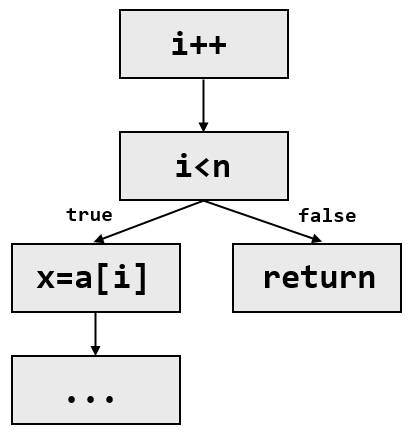
\includegraphics[width=0.3\textwidth]{images/symbolic_execution.png}
		\caption{Ausführungspfade für die symbolische Ausführung einer if-Anweisung}
\end{SCfigure}

Der aktuelle Zustand der Ausführung wird dabei durch zwei verschiedene Strukturen charakterisiert: 
Den Heap, der alle Elemente (engl. heap chunks) des Speichers beinhaltet sowie eine Liste
der geschlussfolgerten Annahmen (engl. assumptions). Bei der Ausführung der Vorbedingungen werden
diese Aussagen nun untersucht und entweder zum Heap hinzugefügt oder zu den Annahmen.

Beim Verstehen dieser Schritte ist die Verifast-Oberfläche sehr hilfreich, da sie den aktuellen
Zustand für einen beliebigen Haltepunkt anzeigen kann. Die folgende Situation zeigt die Ausführung
einer \lstinline{mismatch}-Implementierung bis zum gesetzten Haltepunkt (gelb hervorgehoben).

\begin{center}
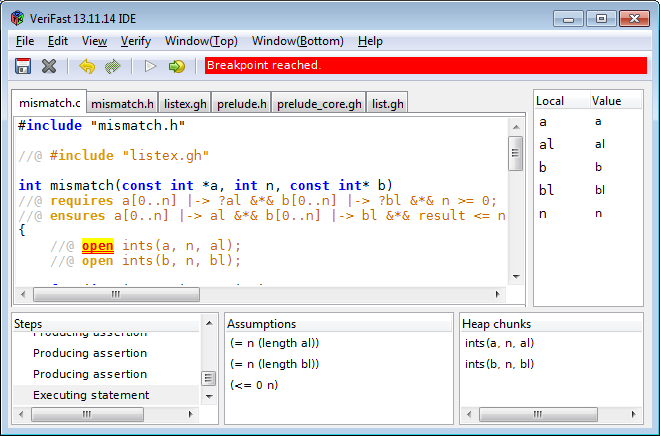
\includegraphics[width=1.0\textwidth]{images/verifast-state-after-precondition.png}
\end{center}

Gut zu erkennen ist, dass logische Ausdrücke wie \(n >= 0\) in die Liste der Annahmen 
(im Bild als \glqq Assumptions\grqq betitelt) aufgenommen wurden. Die \lstinline{ints}-Prädikate hingegen
wurden zum Heap hinzugefügt. Diesen Prozess nennt Verifast \glqq Producing assertion\grqq, wobei sich das Verb
\glqq Producing\grqq auf das Hinzufügen von Elementen zum aktuellen Zustand der symbolischen Ausführung
bezieht.

Das Gegenteil - \glqq Consuming assertion\grqq - findet z.B. beim Verifizieren der Nachbedingungen statt.
Verifast versucht dann alle erforderlichen Aussagen in der Liste der Annahmen bzw. im Heap zu finden
und diese, wenn sie denn passen, zu entfernen. Zusätzlich dazu wird am Ende einer Funktion - beim 
\glqq Leak check\grqq - auch überprüft, dass der Heap (der aktuellen Funktion) leer ist. Ist das nicht 
der Fall so wurde der entsprechende Speicher nicht korrekt bereinigt oder zumindest war Verifast nicht 
in der Lage das Gegenteil zu beweisen.

In dem Fall von mismatch würde Verifast die Heap chunks \lstinline{ints(a, n, al)} sowie
\lstinline{ints(b, n, bl)} beim Konsumieren der Nachbedingung auf dem Heap finden, entfernen und
somit erfolgreich verifizieren können, dass der Speicher so wie vor dem Aufruf vorhanden ist.



\section{Assertions und Ghost-Commands}

Zusicherungen (engl. assertions) und Ghost-Commands sind Annotationen, die direkt in den Implementierungs-Code
geschrieben werden. Assertions stellen sicher, dass der enthaltene Ausdruck wahr ist und sind ein nützliches Hilfsmittel, 
um die Verifizierung besser nachzuvollziehen als auch verständlicher zu machen. Insbesondere dann, wenn das Verifikationswerkzeug 
nicht triviale Schlüsse zieht, ist es von Vorteil Assertions zu ergänzen und im Code zu belassen.

Ghost-Commands hingegen enthalten Anweisungen für die Verifizierung, z.B. das Aufrufen anderer Sprachkonstrukte 
(z.B. Lemmata oder Fixpointfunktionen, siehe \ref{verifizierung:lemma}). Sie helfen dem Werkzeug logische Schlüsse 
zu ziehen, die es alleine nicht tun kann.
\newline
\newline
Der folgende Quellcode zeigt einen Ausschnitt aus einer rekursiven Implementierung für \lstinline{equal} und dient
hier als Anschauungsmaterial für die Erklärung der oben genannten Annotationstypen:

\lstinputlisting[language=C, caption=Rekursive Implementierung für \lstinline{equal} mit Verifast]{codes/equal_recursive_verifast.c}

Diese Implementierung zeigt nur die Abbruchbedingung der Rekursion - ist \lstinline{n == 0}, so sind die
leeren Listen gleich und die Berechnung terminiert. 

Die Zeilen 9 und 10 sind Assertions, die formal beschreiben, dass die induktiven Listen \lstinline{al} und
\lstinline{bl} die Länge 0 haben müssen und somit gleich lang sind. Damit Verifast in der Lage ist das zu
beweisen sind die zwei Ghost-Commands in Zeile 5 und 6 notwendig. Sie öffnen das \lstinline{ints}-Prädikat
und bringen somit dessen Inhalt in die Liste der Annahmen. Erst dadurch ist für Verifast ersichtlich, dass 
\lstinline{n} gleichzusetzen ist mit \texttt{length(al)} und \texttt{length(bl)}. Außerdem produziert
das Öffnen des Prädikats die Formel \lstinline{al = nil} bzw. \lstinline{bl = nil} (siehe Definition
des Prädikats in Listing 3.9 oder 4.2). Damit löst sich die Assertion \lstinline{al == bl} in den
trivialen Vergleich \lstinline{nil == nil} auf.
\newline
\newline
Das Öffnen der Prädikate konsumiert gleichzeitig auch die entsprechenden Heap-Chunks, was jedoch dazu führt,
dass diese beim Produzieren der Nachbedingung fehlen. Sie müssen also vor der \(return\)-Anweisung
wieder geschlossen werden (Zeile 11 und 12), damit sie dann wieder an den Aufrufer zurückgegeben werden können 
- so wie es die Nachbedingung verlangt.

Das Schreiben dieser \(close\)-Annotation ist jedoch oft nicht notwendig, da Verifast sie automatisch
einführt, wenn es sich um ein sogenanntes präzises Prädikat handelt. Darunter versteht Verifast Prädikate mit 
eingehenden und ausgehenden Parametern, die exakt die gleiche Speicherregion repräsentieren. 

\begin{figure}[H]
Die Kennzeichnung als präzises Prädikat geschieht über die Nutzung eines Semikolons bei der Trennung
der Prädikaten-Parameter:

\lstinputlisting[language=C, caption=Präzises Prädikat \lstinline{ints}]{codes/ints_precise_predicate_verifast.c}
\end{figure}
Präzise Prädikate versucht Verifast während der Verifizierung automatisch zu öffnen und ggf. auch zu
schließen. Dadurch ist in der obigen Implementierung das Schreiben der \texttt{close}-Anweisungen
nicht zwingend notwendig.
\newline
\newline
Assertions in ACSL werden genauso notiert wie in Verifast. Ghost-Commands hingegen werden
mit dem Schlüsseltwort \lstinline{ghost} eingeleitet, sind aber generell nicht so oft wie in
Verifast notwendig. Das kommt daher, dass Frama-C aufwendigere Berechnungen durchführt, um
entsprechende logische Schlüsse zu ziehen. Das ist jedoch auch spürbar, wenn man die
Geschwindigkeit der Werkzeuge vergleicht.


\section{Schleifeninvarianten}

schleifeninvarianten in acsl

alle angefassten variablen müssen per assigns erlaubt werden

dann in verifast zeigen

ähnlich, alles muss in invariante defniiert sein, was man benutzen will

toolunterstützung frama-c zeigen und erklären

\section{Lemmata und Axiome}
\label{verifizierung:lemma}

intsinv zeigen mit length

fixpoint nochmal zeigen (take)

erwähnen dass verifast terminierung von fixpount und lemmas prüft

\lstinline{take_one_plus} lemma zeigen

ggf. screenshot hier erst zeigen

erklären wieso es notwendig ist

\section{Speicherprobleme aufdecken}

malloc/free - chunks

zeigen an hand von main-funktion (unit-test)

verifast hilft klar zu dokumentieren wer für speicher verantwortlich ist (rufer oder gerufener)

\section{Überläufe erkennen}

overflow checken

\chapter{Vergleich weiterer Aspekte}


\section{Aliasing}

copy oder move zeigen und unterschied zwischen acsl und verifast

\lstinline{\seperated}



\listoffigures

\end{document}

